\chapter{Teorija igara}

U ovom poglavlju usredotočit ćemo se na igre za
dva igrača koje ne sadrže slučajne elemente.
Cilj nam je pronaći strategiju koje se možemo
držati kako bismo pobijedili u igri
bez obzira na to što protivnik čini,
ako takva strategija postoji.

Ispostavlja se da za takve igre postoji
opća strategija
te da igre možemo analizirati pomoću \key{nim teorije}.
Najprije ćemo analizirati jednostavne igre u kojima
igrači uzimaju štapiće s hrpa,
a nakon toga ćemo strategiju korištenu
u tim igrama generalizirati na druge igre.

\section{Stanja igre}

Razmotrimo igru u kojoj se na početku nalazi
hrpa od $n$ štapića.
Igrači $A$ i $B$ igraju naizmjence,
a igrač $A$ počinje.
U svakom potezu igrač mora uzeti
1, 2 ili 3 štapića s hrpe,
a igrač koji uzme posljednji štapić pobjeđuje u igri.

Na primjer, ako je $n=10$, igra može teći ovako:
\begin{itemize}[noitemsep]
\item Igrač $A$ uzima 2 štapića (ostaje 8 štapića).
\item Igrač $B$ uzima 3 štapića (ostaje 5 štapića).
\item Igrač $A$ uzima 1 štapić (ostaju 4 štapića).
\item Igrač $B$ uzima 2 štapića (ostaju 2 štapića).
\item Igrač $A$ uzima 2 štapića i pobjeđuje.
\end{itemize}

Ova se igra sastoji od stanja $0,1,2,\ldots,n$,
gdje broj stanja odgovara
broju preostalih štapića.

\subsubsection{Pobjednička i gubitnička stanja}

\index{pobjedničko stanje}
\index{gubitničko stanje}

\key{Pobjedničko stanje} je stanje u kojem će
igrač pobijediti u igri ako
igra optimalno,
a \key{gubitničko stanje} je stanje
u kojem će igrač izgubiti igru ako
protivnik igra optimalno.
Ispostavlja se da sva stanja igre možemo
klasificirati tako da je svako stanje ili
pobjedničko ili gubitničko.

U gornjoj igri stanje 0 očito je
gubitničko stanje, jer igrač ne može odigrati
nijedan potez.
Stanja 1, 2 i 3 su pobjednička stanja,
jer možemo uzeti 1, 2 ili 3 štapića
i pobijediti u igri.
Stanje 4 je, s druge strane, gubitničko stanje,
jer svaki potez vodi u stanje koje
je pobjedničko za protivnika.

Općenitije, ako postoji potez koji vodi
iz trenutnog stanja u gubitničko stanje,
trenutno je stanje pobjedničko,
a inače je trenutno stanje gubitničko.
Koristeći to zapažanje, možemo klasificirati sva stanja
igre počevši od gubitničkih stanja u kojima
nema mogućih poteza.

Stanja $0 \ldots 15$ gornje igre
mogu se klasificirati ovako
($W$ označava pobjedničko, a $L$ gubitničko stanje):
\begin{center}
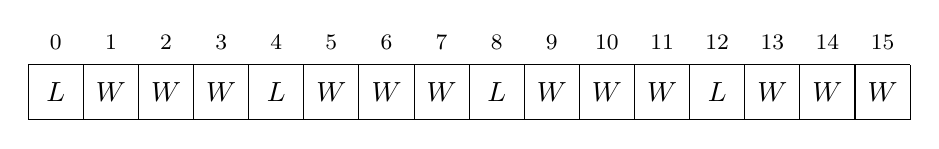
\begin{tikzpicture}[scale=0.7]
\draw (0,0) grid (16,1);

\node at (0.5,0.5) {$L$};
\node at (1.5,0.5) {$W$};
\node at (2.5,0.5) {$W$};
\node at (3.5,0.5) {$W$};
\node at (4.5,0.5) {$L$};
\node at (5.5,0.5) {$W$};
\node at (6.5,0.5) {$W$};
\node at (7.5,0.5) {$W$};
\node at (8.5,0.5) {$L$};
\node at (9.5,0.5) {$W$};
\node at (10.5,0.5) {$W$};
\node at (11.5,0.5) {$W$};
\node at (12.5,0.5) {$L$};
\node at (13.5,0.5) {$W$};
\node at (14.5,0.5) {$W$};
\node at (15.5,0.5) {$W$};

\footnotesize
\node at (0.5,1.4) {$0$};
\node at (1.5,1.4) {$1$};
\node at (2.5,1.4) {$2$};
\node at (3.5,1.4) {$3$};
\node at (4.5,1.4) {$4$};
\node at (5.5,1.4) {$5$};
\node at (6.5,1.4) {$6$};
\node at (7.5,1.4) {$7$};
\node at (8.5,1.4) {$8$};
\node at (9.5,1.4) {$9$};
\node at (10.5,1.4) {$10$};
\node at (11.5,1.4) {$11$};
\node at (12.5,1.4) {$12$};
\node at (13.5,1.4) {$13$};
\node at (14.5,1.4) {$14$};
\node at (15.5,1.4) {$15$};
\end{tikzpicture}
\end{center}

Ovu je igru lako analizirati:
stanje $k$ je gubitničko ako je $k$
djeljiv s 4, a inače je
pobjedničko.
Optimalan način igranja je
da uvijek odaberemo potez nakon kojeg
je broj štapića na hrpi
djeljiv s 4.
Na kraju ne ostaje nijedan štapić i
protivnik je izgubio.

Naravno, ta strategija zahtijeva da
broj štapića \emph{nije} djeljiv s 4
kada je naš potez.
Ako jest, ne možemo ništa učiniti,
i protivnik će pobijediti u igri ako
igra optimalno.

\subsubsection{Graf stanja}

Razmotrimo sada drugu igru sa štapićima,
u kojoj je u svakom stanju $k$ dopušteno uzeti
bilo koji broj $x$ štapića takav da je $x$
manji od $k$ i da dijeli $k$.
Na primjer, u stanju 8 možemo uzeti
1, 2 ili 4 štapića, dok je u stanju 7 jedini
dopušteni potez uzimanje 1 štapića.

Sljedeća slika prikazuje stanja
$1 \ldots 9$ igre kao \key{graf stanja},
čiji su čvorovi stanja, a bridovi potezi između njih:

\begin{center}
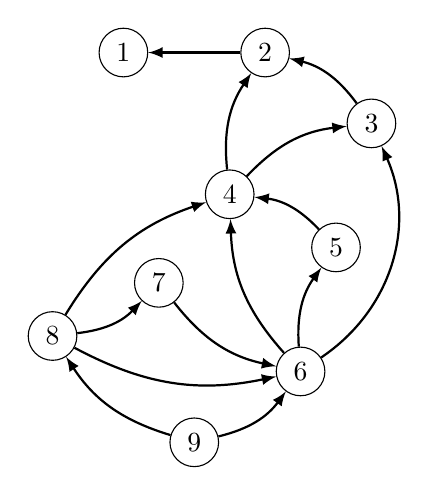
\begin{tikzpicture}[scale=0.9]
\node[draw, circle] (1) at (0,0) {$1$};
\node[draw, circle] (2) at (2,0) {$2$};
\node[draw, circle] (3) at (3.5,-1) {$3$};
\node[draw, circle] (4) at (1.5,-2) {$4$};
\node[draw, circle] (5) at (3,-2.75) {$5$};
\node[draw, circle] (6) at (2.5,-4.5) {$6$};
\node[draw, circle] (7) at (0.5,-3.25) {$7$};
\node[draw, circle] (8) at (-1,-4) {$8$};
\node[draw, circle] (9) at (1,-5.5) {$9$};

\path[draw,thick,->,>=latex] (2) -- (1);
\path[draw,thick,->,>=latex] (3) edge [bend right=20] (2);
\path[draw,thick,->,>=latex] (4) edge [bend left=20] (2);
\path[draw,thick,->,>=latex] (4) edge [bend left=20] (3);
\path[draw,thick,->,>=latex] (5) edge [bend right=20] (4);
\path[draw,thick,->,>=latex] (6) edge [bend left=20] (5);
\path[draw,thick,->,>=latex] (6) edge [bend left=20] (4);
\path[draw,thick,->,>=latex] (6) edge [bend right=40] (3);
\path[draw,thick,->,>=latex] (7) edge [bend right=20] (6);
\path[draw,thick,->,>=latex] (8) edge [bend right=20] (7);
\path[draw,thick,->,>=latex] (8) edge [bend right=20] (6);
\path[draw,thick,->,>=latex] (8) edge [bend left=20] (4);
\path[draw,thick,->,>=latex] (9) edge [bend left=20] (8);
\path[draw,thick,->,>=latex] (9) edge [bend right=20] (6);
\end{tikzpicture}
\end{center}

Završno stanje u ovoj igri uvijek je stanje 1,
koje je gubitničko, jer nema
valjanih poteza.
Klasifikacija stanja $1 \ldots 9$
izgleda ovako:

\begin{center}
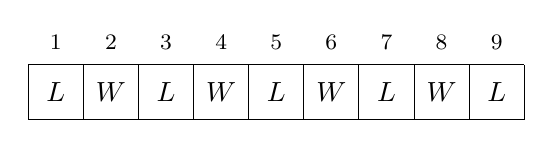
\begin{tikzpicture}[scale=0.7]
\draw (1,0) grid (10,1);

\node at (1.5,0.5) {$L$};
\node at (2.5,0.5) {$W$};
\node at (3.5,0.5) {$L$};
\node at (4.5,0.5) {$W$};
\node at (5.5,0.5) {$L$};
\node at (6.5,0.5) {$W$};
\node at (7.5,0.5) {$L$};
\node at (8.5,0.5) {$W$};
\node at (9.5,0.5) {$L$};

\footnotesize
\node at (1.5,1.4) {$1$};
\node at (2.5,1.4) {$2$};
\node at (3.5,1.4) {$3$};
\node at (4.5,1.4) {$4$};
\node at (5.5,1.4) {$5$};
\node at (6.5,1.4) {$6$};
\node at (7.5,1.4) {$7$};
\node at (8.5,1.4) {$8$};
\node at (9.5,1.4) {$9$};
\end{tikzpicture}
\end{center}

Iznenađujuće, u ovoj su igri
sva stanja s parnim brojem pobjednička,
a sva stanja s neparnim brojem gubitnička.

\section{Igra nim}

\index{igra nim}

\key{Igra nim} jednostavna je igra koja
ima važnu ulogu u teoriji igara,
jer se mnoge druge igre mogu igrati
istom strategijom.
Najprije ćemo se usredotočiti na nim,
a zatim ćemo strategiju generalizirati
na druge igre.

U nimu postoji $n$ hrpa,
a svaka hrpa sadrži neki broj štapića.
Igrači igraju naizmjence,
a u svakom potezu igrač odabire
hrpu koja još sadrži štapiće
i s nje uzima bilo koji broj štapića.
Pobjednik je igrač koji uzme posljednji štapić.

Stanja u nimu su oblika
$[x_1,x_2,\ldots,x_n]$,
gdje $x_k$ označava broj štapića na hrpi $k$.
Na primjer, $[10,12,5]$ je igra u kojoj
postoje tri hrpe s 10, 12 i 5 štapića.
Stanje $[0,0,\ldots,0]$ je gubitničko stanje,
jer nije moguće uzeti nijedan štapić,
te je to uvijek završno stanje.

\subsubsection{Analiza}
\index{nim suma}

Ispostavlja se da bilo koje nim stanje možemo
lako klasificirati izračunom
\key{nim sume} $s = x_1 \oplus x_2 \oplus \cdots \oplus x_n$,
gdje je $\oplus$ operacija xor\footnote{Optimalnu strategiju
za nim objavio je 1901. C. L. Bouton \cite{bou01}.}.
Stanja čija je nim suma 0 su gubitnička stanja,
a sva su ostala stanja pobjednička.
Na primjer, nim suma stanja
$[10,12,5]$ je $10 \oplus 12 \oplus 5 = 3$,
pa je to stanje pobjedničko.

No kako je nim suma povezana s igrom nim?
To možemo objasniti tako da pogledamo kako se nim
suma mijenja kada se nim stanje promijeni.

\textit{Gubitnička stanja:}
Završno stanje $[0,0,\ldots,0]$ je gubitničko stanje,
a njegova je nim suma 0, kao što i očekujemo.
U ostalim gubitničkim stanjima svaki potez vodi u
pobjedničko stanje, jer kada se promijeni jedna vrijednost $x_k$,
mijenja se i nim suma, pa je nim suma
nakon poteza različita od 0.

\textit{Pobjednička stanja:}
U gubitničko stanje možemo prijeći ako
postoji hrpa $k$ za koju je $x_k \oplus s < x_k$.
U tom slučaju možemo uzeti štapiće s
hrpe $k$ tako da ona sadrži $x_k \oplus s$ štapića,
što vodi u gubitničko stanje.
Takva hrpa uvijek postoji, i to ona za koju $x_k$
ima bit jedan na poziciji krajnje lijevog
bita jedan u $s$.

Kao primjer razmotrimo stanje $[10,12,5]$.
To je stanje pobjedničko,
jer je njegova nim suma 3.
Stoga mora postojati potez koji
vodi u gubitničko stanje.
Sljedeće ćemo pronaći takav potez.

Nim suma stanja izgleda ovako:

\begin{center}
\begin{tabular}{r|r}
10 & \texttt{1010} \\
12 & \texttt{1100} \\
5 & \texttt{0101} \\
\hline
3 & \texttt{0011} \\
\end{tabular}
\end{center}

U ovom slučaju hrpa s 10 štapića
jedina je hrpa koja ima bit jedan
na poziciji krajnje lijevog
bita jedan u nim sumi:

\begin{center}
\begin{tabular}{r|r}
10 & \texttt{10\underline{1}0} \\
12 & \texttt{1100} \\
5 & \texttt{0101} \\
\hline
3 & \texttt{00\underline{1}1} \\
\end{tabular}
\end{center}

Nova veličina hrpe mora biti
$10 \oplus 3 = 9$,
pa ćemo uzeti samo jedan štapić.
Nakon toga stanje će biti $[9,12,5]$,
koje je gubitničko:

\begin{center}
\begin{tabular}{r|r}
9 & \texttt{1001} \\
12 & \texttt{1100} \\
5 & \texttt{0101} \\
\hline
0 & \texttt{0000} \\
\end{tabular}
\end{center}

\subsubsection{Misère igra}

\index{misère igra}

U \key{misère igri} cilj igre
je suprotan,
pa igrač koji uzme posljednji štapić
gubi igru.
Ispostavlja se da se misère nim može
optimalno igrati gotovo isto kao i standardni nim.

Ideja je misère igru najprije igrati
kao standardnu igru, ali promijeniti strategiju
na kraju igre.
Novu strategiju uvodimo u situaciji
u kojoj bi nakon sljedećeg poteza svaka hrpa
sadržavala najviše jedan štapić.

U standardnoj igri trebamo odabrati potez
nakon kojeg postoji paran broj hrpa s jednim štapićem.
U misère igri, međutim, odabiremo potez tako da
postoji neparan broj hrpa s jednim štapićem.

Ta strategija radi zato što se stanje u kojem se
strategija mijenja uvijek pojavi u igri,
a to je stanje pobjedničko, jer
sadrži točno jednu hrpu s više od jednog štapića
pa nim suma nije 0.

\section{Sprague–Grundyjev teorem}

\index{Sprague–Grundyjev teorem}

\key{Sprague–Grundyjev teorem}\footnote{Teorem su
neovisno otkrili R. Sprague \cite{spr35} i P. M. Grundy \cite{gru39}.} generalizira
strategiju korištenu u nimu na sve igre koje zadovoljavaju
sljedeće zahtjeve:

\begin{itemize}[noitemsep]
\item Postoje dva igrača koji igraju naizmjence.
\item Igra se sastoji od stanja, a mogući potezi
u nekom stanju ne zavise od toga čiji je potez.
\item Igra završava kada igrač ne može odigrati potez.
\item Igra sigurno prije ili kasnije završava.
\item Igrači imaju potpunu informaciju o
stanjima i dopuštenim potezima, a u igri nema slučajnosti.
\end{itemize}
Ideja je za svako stanje igre izračunati
Grundyjev broj koji odgovara broju
štapića na nim hrpi.
Kada znamo Grundyjeve brojeve svih stanja,
igru možemo igrati kao igru nim.

\subsubsection{Grundyjevi brojevi}

\index{Grundyjev broj}
\index{funkcija mex}

\key{Grundyjev broj} stanja igre jest
\[\textrm{mex}(\{g_1,g_2,\ldots,g_n\}),\]
gdje su $g_1,g_2,\ldots,g_n$ Grundyjevi brojevi
stanja u koja možemo prijeći,
a funkcija mex daje najmanji
nenegativni broj koji nije u skupu.
Na primjer, $\textrm{mex}(\{0,1,3\})=2$.
Ako u nekom stanju nema mogućih poteza,
njegov je Grundyjev broj 0, jer je
$\textrm{mex}(\emptyset)=0$.

Na primjer, u grafu stanja
\begin{center}
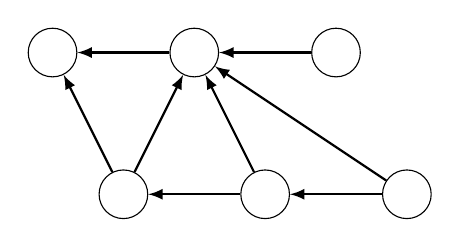
\begin{tikzpicture}[scale=0.9]
\node[draw, circle] (1) at (0,0) {\phantom{0}};
\node[draw, circle] (2) at (2,0) {\phantom{0}};
\node[draw, circle] (3) at (4,0) {\phantom{0}};
\node[draw, circle] (4) at (1,-2) {\phantom{0}};
\node[draw, circle] (5) at (3,-2) {\phantom{0}};
\node[draw, circle] (6) at (5,-2) {\phantom{0}};

\path[draw,thick,->,>=latex] (2) -- (1);
\path[draw,thick,->,>=latex] (3) -- (2);
\path[draw,thick,->,>=latex] (5) -- (4);
\path[draw,thick,->,>=latex] (6) -- (5);
\path[draw,thick,->,>=latex] (4) -- (1);
\path[draw,thick,->,>=latex] (4) -- (2);
\path[draw,thick,->,>=latex] (5) -- (2);
\path[draw,thick,->,>=latex] (6) -- (2);
\end{tikzpicture}
\end{center}
Grundyjevi brojevi izgledaju ovako:
\begin{center}
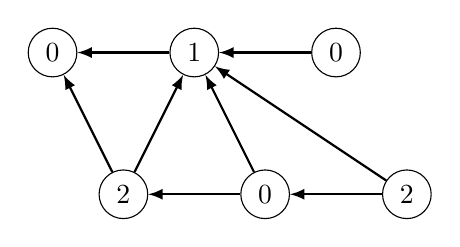
\begin{tikzpicture}[scale=0.9]
\node[draw, circle] (1) at (0,0) {0};
\node[draw, circle] (2) at (2,0) {1};
\node[draw, circle] (3) at (4,0) {0};
\node[draw, circle] (4) at (1,-2) {2};
\node[draw, circle] (5) at (3,-2) {0};
\node[draw, circle] (6) at (5,-2) {2};

\path[draw,thick,->,>=latex] (2) -- (1);
\path[draw,thick,->,>=latex] (3) -- (2);
\path[draw,thick,->,>=latex] (5) -- (4);
\path[draw,thick,->,>=latex] (6) -- (5);
\path[draw,thick,->,>=latex] (4) -- (1);
\path[draw,thick,->,>=latex] (4) -- (2);
\path[draw,thick,->,>=latex] (5) -- (2);
\path[draw,thick,->,>=latex] (6) -- (2);
\end{tikzpicture}
\end{center}
Grundyjev broj gubitničkog stanja je 0,
a Grundyjev broj pobjedničkog stanja je
pozitivan broj.

Grundyjev broj stanja odgovara
broju štapića na nim hrpi.
Ako je Grundyjev broj 0, možemo prijeći samo u
stanja čiji su Grundyjevi brojevi pozitivni,
a ako je Grundyjev broj $x>0$, možemo prijeći
u stanja čiji Grundyjevi brojevi uključuju sve brojeve
$0,1,\ldots,x-1$.

Kao primjer razmotrimo igru u kojoj
igrači pomiču figuru po labirintu.
Svaki je kvadrat labirinta ili pod ili zid.
U svakom potezu igrač mora pomaknuti
figuru za neki broj
koraka ulijevo ili prema gore.
Pobjednik igre je igrač koji
odigra posljednji potez.

Sljedeća slika prikazuje moguće početno stanje
igre, gdje @ označava figuru, a *
označava kvadrat na koji se ona može pomaknuti.

\begin{center}
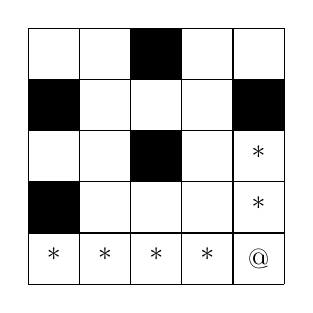
\begin{tikzpicture}[scale=.65]
  \begin{scope}
    \fill [color=black] (0, 1) rectangle (1, 2);
    \fill [color=black] (0, 3) rectangle (1, 4);
    \fill [color=black] (2, 2) rectangle (3, 3);
    \fill [color=black] (2, 4) rectangle (3, 5);
    \fill [color=black] (4, 3) rectangle (5, 4);

    \draw (0, 0) grid (5, 5);
    
    \node at (4.5,0.5) {@};
    \node at (3.5,0.5) {*};
    \node at (2.5,0.5) {*};
    \node at (1.5,0.5) {*};
    \node at (0.5,0.5) {*};
    \node at (4.5,1.5) {*};
    \node at (4.5,2.5) {*};
    
  \end{scope}
\end{tikzpicture}
\end{center}

Stanja igre su svi kvadrati poda
u labirintu.
U gornjem labirintu Grundyjevi brojevi
izgledaju ovako:

\begin{center}
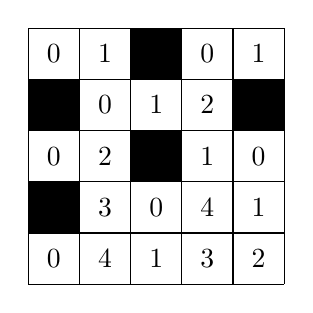
\begin{tikzpicture}[scale=.65]
  \begin{scope}
    \fill [color=black] (0, 1) rectangle (1, 2);
    \fill [color=black] (0, 3) rectangle (1, 4);
    \fill [color=black] (2, 2) rectangle (3, 3);
    \fill [color=black] (2, 4) rectangle (3, 5);
    \fill [color=black] (4, 3) rectangle (5, 4);

    \draw (0, 0) grid (5, 5);
    
    \node at (0.5,4.5) {0};
    \node at (1.5,4.5) {1};
    \node at (2.5,4.5) {};
    \node at (3.5,4.5) {0};
    \node at (4.5,4.5) {1};

    \node at (0.5,3.5) {};
    \node at (1.5,3.5) {0};
    \node at (2.5,3.5) {1};
    \node at (3.5,3.5) {2};
    \node at (4.5,3.5) {};

    \node at (0.5,2.5) {0};
    \node at (1.5,2.5) {2};
    \node at (2.5,2.5) {};
    \node at (3.5,2.5) {1};
    \node at (4.5,2.5) {0};

    \node at (0.5,1.5) {};
    \node at (1.5,1.5) {3};
    \node at (2.5,1.5) {0};
    \node at (3.5,1.5) {4};
    \node at (4.5,1.5) {1};

    \node at (0.5,0.5) {0};
    \node at (1.5,0.5) {4};
    \node at (2.5,0.5) {1};
    \node at (3.5,0.5) {3};
    \node at (4.5,0.5) {2};
  \end{scope}
\end{tikzpicture}
\end{center}

Dakle, svako stanje igre s labirintom
odgovara jednoj hrpi u igri nim.
Na primjer, Grundyjev broj
donjeg desnog kvadrata je 2,
pa je to pobjedničko stanje.
Možemo doći u gubitničko stanje i
pobijediti u igri pomicanjem
ili četiri koraka ulijevo ili
dva koraka prema gore.

Primijetimo da je, drugačije nego u izvornoj igri nim,
moguće prijeći u stanje čiji je
Grundyjev broj veći od Grundyjeva broja
trenutnog stanja.
Protivnik, međutim, uvijek može odabrati potez
koji poništava takav potez, pa nije moguće
umaknuti iz gubitničkog stanja.

\subsubsection{Podigre}

Sljedeće ćemo pretpostaviti da se naša igra sastoji
od podigara te da u svakom potezu igrač
najprije odabire podigru, a zatim potez u toj podigri.
Igra završava kada nije moguće odigrati nijedan potez
ni u jednoj podigri.

U tom slučaju Grundyjev broj igre
jest nim suma Grundyjevih brojeva podigara.
Igra se može igrati kao nim tako da izračunamo
sve Grundyjeve brojeve podigara, a zatim njihovu nim sumu.

Kao primjer razmotrimo igru koja se sastoji
od tri labirinta.
U toj igri igrač u svakom potezu odabire jedan
od labirinata i zatim pomiče figuru u tom labirintu.
Pretpostavimo da je početno stanje igre sljedeće:

\begin{center}
\begin{tabular}{ccc}
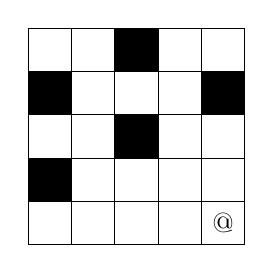
\begin{tikzpicture}[scale=.55]
  \begin{scope}
    \fill [color=black] (0, 1) rectangle (1, 2);
    \fill [color=black] (0, 3) rectangle (1, 4);
    \fill [color=black] (2, 2) rectangle (3, 3);
    \fill [color=black] (2, 4) rectangle (3, 5);
    \fill [color=black] (4, 3) rectangle (5, 4);

    \draw (0, 0) grid (5, 5);

    \node at (4.5,0.5) {@};

    \end{scope}
\end{tikzpicture}
&
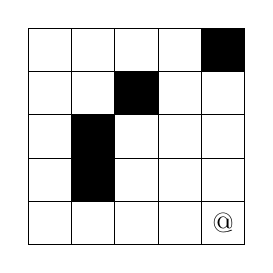
\begin{tikzpicture}[scale=.55]
  \begin{scope}
    \fill [color=black] (1, 1) rectangle (2, 3);
    \fill [color=black] (2, 3) rectangle (3, 4);
    \fill [color=black] (4, 4) rectangle (5, 5);

    \draw (0, 0) grid (5, 5);
    
    \node at (4.5,0.5) {@};

  \end{scope}
\end{tikzpicture}
&
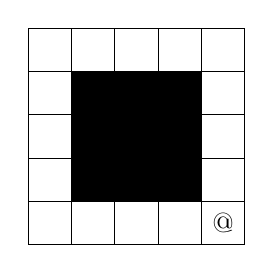
\begin{tikzpicture}[scale=.55]
  \begin{scope}
    \fill [color=black] (1, 1) rectangle (4, 4);

    \draw (0, 0) grid (5, 5);
    
    \node at (4.5,0.5) {@};
  \end{scope}
\end{tikzpicture}
\end{tabular}
\end{center}

Grundyjevi brojevi labirinata izgledaju ovako:

\begin{center}
\begin{tabular}{ccc}
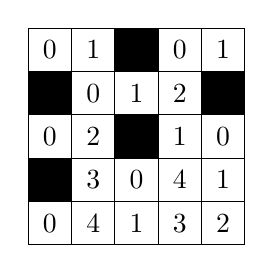
\begin{tikzpicture}[scale=.55]
  \begin{scope}
    \fill [color=black] (0, 1) rectangle (1, 2);
    \fill [color=black] (0, 3) rectangle (1, 4);
    \fill [color=black] (2, 2) rectangle (3, 3);
    \fill [color=black] (2, 4) rectangle (3, 5);
    \fill [color=black] (4, 3) rectangle (5, 4);

    \draw (0, 0) grid (5, 5);

    \node at (0.5,4.5) {0};
    \node at (1.5,4.5) {1};
    \node at (2.5,4.5) {};
    \node at (3.5,4.5) {0};
    \node at (4.5,4.5) {1};

    \node at (0.5,3.5) {};
    \node at (1.5,3.5) {0};
    \node at (2.5,3.5) {1};
    \node at (3.5,3.5) {2};
    \node at (4.5,3.5) {};

    \node at (0.5,2.5) {0};
    \node at (1.5,2.5) {2};
    \node at (2.5,2.5) {};
    \node at (3.5,2.5) {1};
    \node at (4.5,2.5) {0};

    \node at (0.5,1.5) {};
    \node at (1.5,1.5) {3};
    \node at (2.5,1.5) {0};
    \node at (3.5,1.5) {4};
    \node at (4.5,1.5) {1};

    \node at (0.5,0.5) {0};
    \node at (1.5,0.5) {4};
    \node at (2.5,0.5) {1};
    \node at (3.5,0.5) {3};
    \node at (4.5,0.5) {2};
    \end{scope}
\end{tikzpicture}
&
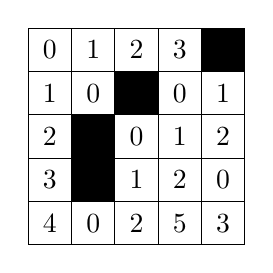
\begin{tikzpicture}[scale=.55]
  \begin{scope}
    \fill [color=black] (1, 1) rectangle (2, 3);
    \fill [color=black] (2, 3) rectangle (3, 4);
    \fill [color=black] (4, 4) rectangle (5, 5);

    \draw (0, 0) grid (5, 5);

    \node at (0.5,4.5) {0};
    \node at (1.5,4.5) {1};
    \node at (2.5,4.5) {2};
    \node at (3.5,4.5) {3};
    \node at (4.5,4.5) {};

    \node at (0.5,3.5) {1};
    \node at (1.5,3.5) {0};
    \node at (2.5,3.5) {};
    \node at (3.5,3.5) {0};
    \node at (4.5,3.5) {1};

    \node at (0.5,2.5) {2};
    \node at (1.5,2.5) {};
    \node at (2.5,2.5) {0};
    \node at (3.5,2.5) {1};
    \node at (4.5,2.5) {2};

    \node at (0.5,1.5) {3};
    \node at (1.5,1.5) {};
    \node at (2.5,1.5) {1};
    \node at (3.5,1.5) {2};
    \node at (4.5,1.5) {0};

    \node at (0.5,0.5) {4};
    \node at (1.5,0.5) {0};
    \node at (2.5,0.5) {2};
    \node at (3.5,0.5) {5};
    \node at (4.5,0.5) {3};
  \end{scope}
\end{tikzpicture}
&
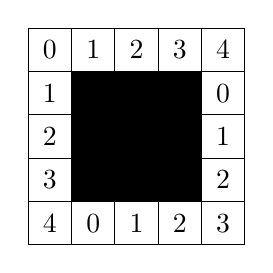
\begin{tikzpicture}[scale=.55]
  \begin{scope}
    \fill [color=black] (1, 1) rectangle (4, 4);

    \draw (0, 0) grid (5, 5);

    \node at (0.5,4.5) {0};
    \node at (1.5,4.5) {1};
    \node at (2.5,4.5) {2};
    \node at (3.5,4.5) {3};
    \node at (4.5,4.5) {4};

    \node at (0.5,3.5) {1};
    \node at (1.5,3.5) {};
    \node at (2.5,3.5) {};
    \node at (3.5,3.5) {};
    \node at (4.5,3.5) {0};

    \node at (0.5,2.5) {2};
    \node at (1.5,2.5) {};
    \node at (2.5,2.5) {};
    \node at (3.5,2.5) {};
    \node at (4.5,2.5) {1};

    \node at (0.5,1.5) {3};
    \node at (1.5,1.5) {};
    \node at (2.5,1.5) {};
    \node at (3.5,1.5) {};
    \node at (4.5,1.5) {2};

    \node at (0.5,0.5) {4};
    \node at (1.5,0.5) {0};
    \node at (2.5,0.5) {1};
    \node at (3.5,0.5) {2};
    \node at (4.5,0.5) {3};
  \end{scope}
\end{tikzpicture}
\end{tabular}
\end{center}

U početnom stanju nim suma Grundyjevih brojeva
jest $2 \oplus 3 \oplus 3 = 2$, pa
prvi igrač može pobijediti u igri.
Jedan optimalan potez je pomak dva koraka prema gore
u prvom labirintu, čime nastaje nim suma
$0 \oplus 3 \oplus 3 = 0$.

\subsubsection{Grundyjeva igra}

Ponekad potez u igri dijeli igru
na podigre koje su međusobno neovisne.
U tom je slučaju Grundyjev broj igre

\[\textrm{mex}(\{g_1, g_2, \ldots, g_n \}),\]
gdje je $n$ broj mogućih poteza i
\[g_k = a_{k,1} \oplus a_{k,2} \oplus \ldots \oplus a_{k,m},\]
gdje potez $k$ stvara podigre s
Grundyjevim brojevima $a_{k,1},a_{k,2},\ldots,a_{k,m}$.

\index{Grundyjeva igra}

Primjer takve igre je \key{Grundyjeva igra}.
Na početku postoji jedna hrpa koja sadrži $n$ štapića.
U svakom potezu igrač odabire hrpu i dijeli
je na dvije neprazne hrpe tako da su hrpe
različite veličine.
Igrač koji odigra posljednji potez pobjeđuje u igri.

Neka je $f(n)$ Grundyjev broj hrpe
koja sadrži $n$ štapića.
Grundyjev broj možemo izračunati prolaskom
kroz sve načine na koje hrpu možemo podijeliti na
dvije hrpe.
Na primjer, kada je $n=8$, mogućnosti
su $1+7$, $2+6$ i $3+5$, pa je
\[f(8)=\textrm{mex}(\{f(1) \oplus f(7), f(2) \oplus f(6), f(3) \oplus f(5)\}).\]

U ovoj se igri vrijednost $f(n)$ temelji na vrijednostima
$f(1),\ldots,f(n-1)$.
Bazni slučajevi su $f(1)=f(2)=0$,
jer nije moguće podijeliti hrpe
od 1 i 2 štapića.
Prvi Grundyjevi brojevi su:
\[
\begin{array}{lcl}
f(1) & = & 0 \\
f(2) & = & 0 \\
f(3) & = & 1 \\
f(4) & = & 0 \\
f(5) & = & 2 \\
f(6) & = & 1 \\
f(7) & = & 0 \\
f(8) & = & 2 \\
\end{array}
\]
Grundyjev broj za $n=8$ je 2,
pa je moguće pobijediti u igri.
Pobjednički potez je stvoriti hrpe
$1+7$, jer je $f(1) \oplus f(7) = 0$.

